\documentclass{article}
\usepackage{graphicx}
\usepackage{algorithm}
\usepackage[noend]{algorithmic}
\usepackage{subfigure}
\usepackage{amssymb, amsmath, graphicx, charter, latexsym}
\usepackage{layouts}
\usepackage[letterpaper]{geometry}
\usepackage{enumerate}
\usepackage{epstopdf}
\usepackage{ragged2e}
%\usepackage{times}
\usepackage{mathtools}
%\usepackage[scaled]{helvet}
\usepackage{mathptmx}
\usepackage{verbatim}
\usepackage{listings}
\usepackage{siunitx}
\usepackage{booktabs}

\lstset{
basicstyle=\ttfamily,
}
\lstMakeShortInline|

\begin{document}

\title{\bfseries ECEN 689 -- Real-Time Wireless Networks: Project 2\\
Scheduling for Uplink Transmissions with Point Coordination Function}
\date{Due on 4/1}
\author{%
Ping-Chun Hsieh\\
\texttt{lleyfede@tamu.edu}
\and
Tao Zhao\\
\texttt{alick@tamu.edu}
\and
Dongni Han\\
\texttt{handongni2015@tamu.edu}
}
\maketitle

\section*{Terminology}

In our report, we use AP or ``server'' to denote the WiFi access point, and
``client'' to denote the terminal device such as a mobile phone, a tablet, and
so on. Throughout our simulation, we let node $0$ be the server, and the other nodes be the clients. The basic time unit for packet transmission is called \emph{slot}, which should be greater than a round-trip time (RTT). For real-time traffic, we group an integer number (denoted by $T$) of slots into an \emph{interval}, which is the relative deadline of the packets.

\section{Background}

We consider a wireless network of one AP and $K$ clients,
where $K\ge1$. We consider uplink transmission with point coordination function (PCF).
In PCF mode, the AP has full control over channel allocation. In the beginning of each interval, each client generates a random number of packets and waits for channel access that is fully controlled by the AP. Since the packets are generated and queued on the client's side, the AP needs to collect the queue information of the clients to make scheduling decisions.

In this project we consider a baseline policy, where the AP collects the queue
information by polling each client one by one for the number of data packets it
generates.
After all clients are polled, the AP knows the number of packets at each client,
then schedules one of the clients in each time slot for actual uplink data transmission.

\section{Implementation in NS-2}
\label{section: ns2}

Because there is no PCF functions available in 802.11 Mac module in ns-2, and we
prefer to make minimal changes to the 802.11 Mac implementation itself, we
implement the PCF functions with the baseline policy in the application layer,
where we define the \lstinline|hdr_swifi| packet header and the \lstinline|SWiFiAgent| class.

In the beginning of simulation, one node becomes the AP by issuing the
\lstinline|server| command. For example,
\lstinline|$sw(0) server| makes the zeroth node the server.
Client registration is done by the \lstinline|register|
command. For instance, \lstinline|$sw_(0) register 1 0.5|
registers node 1 as a client with channel reliability $0.5$.%
\footnote{We use a lookup table to map the distance between the server and the
client to the channel reliability based on the result of reliability measurement
in project 1.}

\newcommand\CC{C\nolinebreak[4]\hspace{-.05em}\raisebox{0.3ex}{++}}

In the beginning of each interval, the AP calls |boi|, which stands for
``beginning of interval'', to reset its internal state and packet counters.
Each client generates a random number of packets from a uniform distribution,
and uses the |pour| command to make it available from Tcl to \CC.

In each time slot, the AP executes the \lstinline |poll| command.
Based on its state, it either sends a certain type of poll packet, or idle.
In the beginning of each interval, the AP is in the |SWiFi_POLL_NUM| state,
and calls \lstinline |scheduleRoundRobin(false)| to find the next client
to poll the number of new packets
in the order of initial registration. Here |false| means
once all clients have been scheduled exactly once, no one will be scheduled
again, instead of scheduling from the first one repeatedly.
The AP sends a |SWiFi_PKT_POLL_NUM| packet to the target client.

When the client receives the |SWiFi_PKT_POLL_NUM| packet, it replies a
|SWiFi_PKT_NUM_UL| packet with its number of packets in the packet header.
The number (denoted by $X_n$) is the number
of newly generated packets in this interval for real-time traffic, while it is
the number of total generated packets up to now for non-real-time traffic.
When the AP receives the packet, it acquires the number, and calculates the
queue length of the client.
For real-time traffic, the queue length is the same
as the received number. For non-real-time traffic,
in order to derive the real queue length of each client, the AP needs to keep track of the total number of received packets (denoted by $Y_n$) from each client $n$, and then calculates the queue length as $(X_n - Y_n)$ for each client $n$.
If either the transmission of \lstinline|SWiFi_PKT_POLL_NUM| or
\lstinline|SWiFi_PKT_NUM_UL| fails, the AP will retransmit the
\lstinline|SWiFi_PKT_POLL_NUM| packet again to the same client in the next slot. 

After all clients have been polled for their numbers of packets,
the |SWiFi_POLL_NUM| ends and the AP
goes into the |SWiFi_POLL_DATA| state, where actual data packets are polled.
In each slot, the AP applies the Max-Weight policy, which schedules the client
that maximizes the product of its queue length and the channel reliability
in our implementation.

The AP sends a \lstinline|SWiFi_PKT_POLL_DATA| packet to the target client to provide access to the channel.
Note that we put the expected packet ID in the header of |SWiFi_PKT_POLL_DATA| packets
so that the target client knows which packet to transmit and the previous
packets are delivered once it receives the |SWiFi_PKT_POLL_DATA| packet.
This is a better solution than an additional application-layer ACK from  the AP
because the latter needs more time and is still unreliable when the channel is
bad.
The scheduled client's data packet is of type \lstinline|SWiFi_PKT_DATA_UL|.
If the AP receives the data packet successfully, the AP will decrease the queue length by 1. If either the transmission of data polling or the data packet fails, the AP will stay with the same schedule in the next slot (suppose the next slot is not the end of the interval).

If the AP already receives all the packets available in the current interval,
it will go to the idle state |SWiFi_POLL_IDLE| until the start of the next interval.
No packet is transmitted in this state.
On the other hand, for real-time traffic,
if some packets are not delivered within the interval, they will be dropped.

Table~\ref{tab:packet} summarizes the four packet types used in our
implementation, and Figure ~\ref{fig:packet} shows their packet structures.
Table~\ref{tab:state} summarizes the states of the AP in PCF mode,
and state transitions are illustrated in Figure~\ref{fig:state}.

\begin{table}[htbp]
   \centering
   \caption{Packet types.}
   \label{tab:packet}
   \begin{tabular}{| l | l |}
      \hline
      Packet Type  &  Meaning\\ \hline
      \lstinline |SWiFi_PKT_POLL_NUM| & Poll number of packets in uplink\\ \hline 
      \lstinline |SWiFi_PKT_POLL_DATA|  & Poll data packet transmission in uplink\\ \hline 
      \lstinline |SWiFi_PKT_NUM_UL| & Packet in uplink that carries number of packets at client\\ \hline 
      \lstinline |SWiFi_PKT_DATA_UL| & Data packet in uplink (client to AP)\\  
     \hline
   \end{tabular}
\end{table}
 
\begin{table}[h!]
   \centering
   \caption{Poll states.}
   \label{tab:state}
   \begin{tabular}{| l | l |}
      \hline
      Poll State  &  Meaning\\ \hline
      \lstinline |SWiFi_POLL_NONE| & Uninitialized \\ \hline 
      \lstinline |SWiFi_POLL_NUM|  & Poll the number of packets\\ \hline 
      \lstinline |SWiFi_POLL_DATA| & Poll a data packet\\ \hline 
      \lstinline |SWiFi_POLL_IDLE| & Idle\\  
     \hline
   \end{tabular}
\end{table}

\begin{figure}[htbp]
\centering
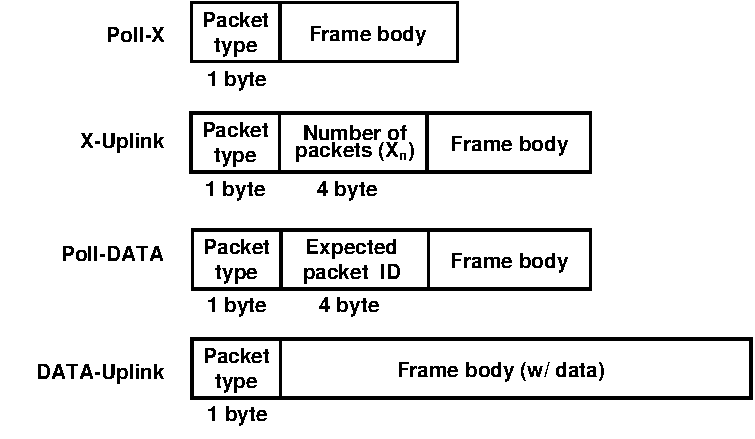
\includegraphics[scale=0.6]{header.pdf}
\caption{Packet structures.}
\label{fig:packet}
\end{figure}


\begin{figure}[htbp]
\centering
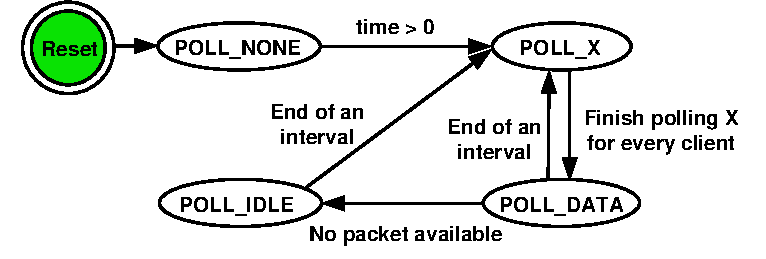
\includegraphics[scale=0.8]{state_machine.pdf}
\caption{State transitions of the AP.}
\label{fig:state}
\end{figure}


\section{Simulation Results}
\begin{table}[htbp]
\centering
    \caption{Parameters of the wireless channel.}
    \vspace{2mm}
    \begin{tabular}{ | l | l | }
    \hline
    Item & Value \\ \hline
    Path loss exponent & 2.0  \\ \hline
    Shadowing deviation & \SI{4.0}{dB} \\ \hline
    Reference distance & \SI{1.0}{m} \\
    \hline
\end{tabular}
\label{table: channel}
\end{table}
Throughout the simulation, we consider a fully-symmetric network with one AP and 2 clients. We use the shadowing module as the wireless channel. The parameters of the channel are summarized in Table \ref{table: channel}. The transmitter power level is \SI{1}{W}. The channel reliability can be changed by varying the distance between the AP and the clients. In our simulation, we set the distance between the AP and a client to be \SI{1}{m} when creating a reliable channel. For an unreliable channel with $p_n\approx 0.57$, the corresponding distance is \SI{1000}{m}. 

\begin{table}[htbp]
\centering
\caption{Parameters of the 802.11b MAC.}
    \vspace{2mm}
    \begin{tabular}{ | l | l | }
    \hline
    Item & Value \\ \hline
    Data rate & \SI{11}{Mb/s}  \\ \hline
    Basic rate & \SI{1}{Mb/s}  \\ \hline
    PLCP data rate & \SI{1}{Mb/s}  \\ \hline 
    Preamble length & \SI{144}{bits} \\ \hline
    Slot time & \SI{20}{\mu s} \\ \hline
    SIFS & \SI{10}{\mu s} \\
    \hline
\end{tabular}
\label{table: mac}
\end{table}

For the medium access control (MAC) layer, we use the 802.11 module built in ns-2. Following the IEEE 802.11b standard, the MAC layer parameters are chosen as in Table \ref{table: mac}. Besides, the automatic retry function built in 802.11 is disabled, i.e. \lstinline|ShortRetryLimit_| and \lstinline|LongRetryLimit_| are set to be 0 in the Tcl domain, to avoid channel congestion due to uncontrollable retransmission in the MAC layer.

Throughout the simulation, a slot is chosen to be $\SI{10}{ms}$, which is much
longer than a RTT ($\approx\SI{1.63}{ms}$), to provide enough margin for packet
delivery. We consider random packet arrivals. The number of packets generated in
an interval follows discrete uniform distribution that ranges between 0 and
$N_{max}$.

To evaluate the performance of the baseline policy, We use the average number of
delivered packets in an interval as the main performance metric. It corresponds
to the timely-throughput for real-time traffic, and is simply the throughput for
non-real-time traffic. The final result is the average of 10 runs under each
set of parameters.

\label{section: simulation}
\subsection{Network Capacity}
We first study the network capacity with different packet generation rates under the baseline policy. Let $T=10$ and the channels be reliable, i.e. $p_1 = p_2 = 1$.
We measure the average network throughput (denoted by $\bar{R}$) with different $N_{max}$.

In the non-real-time scenario, Figure \ref{nonrealtime_throughput_randmax} shows the system throughput for $N_{max}$ between 1 and 12. We can see that the maximum achievable throughput is 8, less than $T$. This is because the AP has to collect the queue information in the polling phase, which lasts for 2 slots in every interval. Therefore, polling indeed reduces the network capacity. Moreover, the dashed line shows the expected network throughput if there is no randomness in packet generation. Thus, for non-real-time traffic, randomness in packet generation does not affect the network throughput.
\begin{figure}[htbp]
\centering
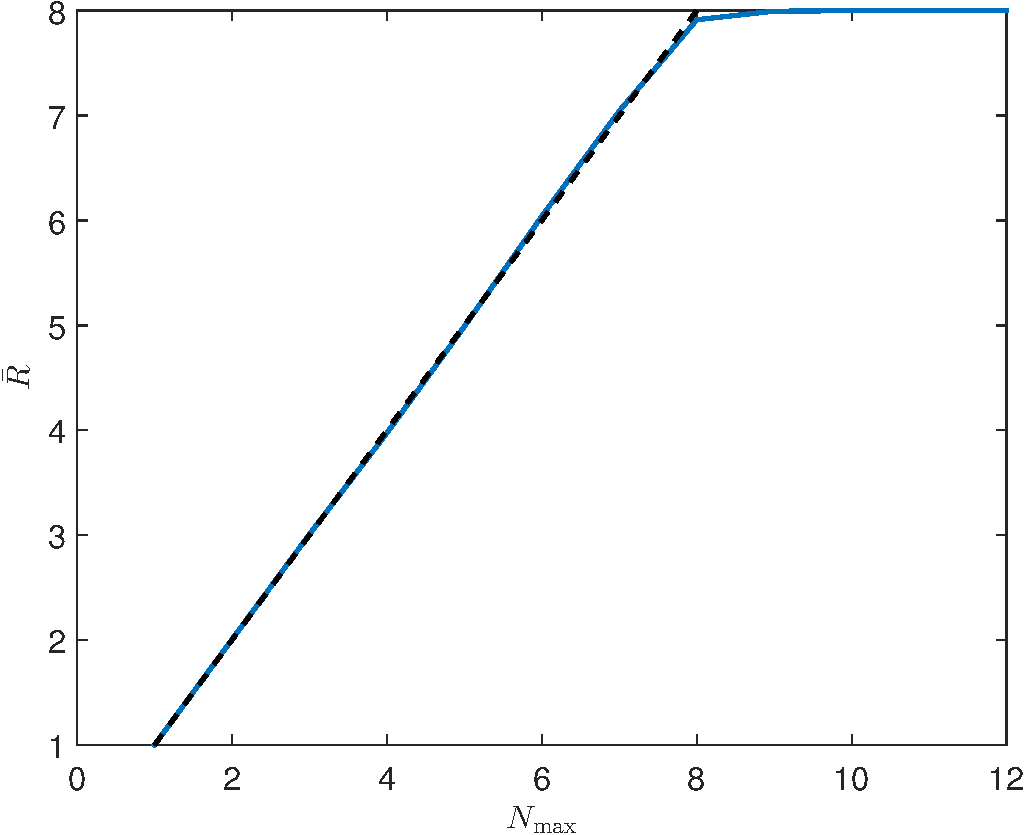
\includegraphics[width=.6\textwidth]{nonrealtime_throughput_randmax.pdf}
\caption{Network throughput versus $N_{max}$ with non-real-time traffic}
\label{nonrealtime_throughput_randmax}
\end{figure}

For real-time traffic, the network throughput is shown in Figure \ref{realtime_throughput_randmax}. Compared to the non-real-time case, the network throughput with real-time traffic is smaller when $N_{max}\geq 5$. This is because packets may expire when the total packets generated in an interval is larger than 8, which is the length of the scheduling phase. Therefore, in addition to polling overhead, packet deadline can further reduce the network throughput. 

\begin{figure}[htbp]
\centering
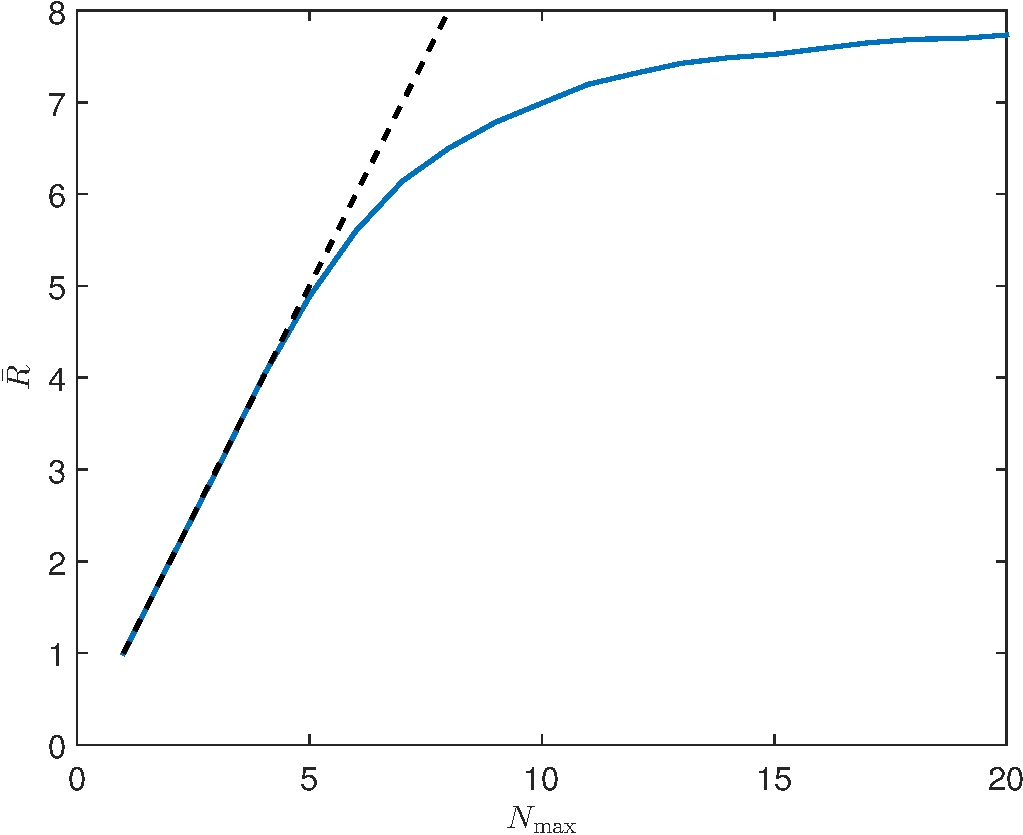
\includegraphics[width=.6\textwidth]{realtime_throughput_randmax.pdf}
\caption{Network throughput versus $N_{max}$ with real-time traffic}
\label{realtime_throughput_randmax}
\end{figure}

\subsection{Choice of Interval Length}
We study the how the choice of $T$ affects the network throughput. Choose $N_{max}=2$ and $p_1 = p_2 = 0.57$. Figure \ref{nonrealtime_throughput_T} shows the network throughput with different interval length in the non-real-time scenario. The total throughput is very low when $T=4$ because the polling overhead is particularly significant for small $T$. Moreover, since larger $T$ implies more available slots to the scheduling phase, the system throughput should increase with interval length. 

%For non-real-time traffic, according to , T ranges from 4 to 16. We can conclude that interval should be long enough to guarantee deliveries. If interval is too short, AP will not have enough time slots to poll data to clients. 

\begin{figure}[htbp]
\centering
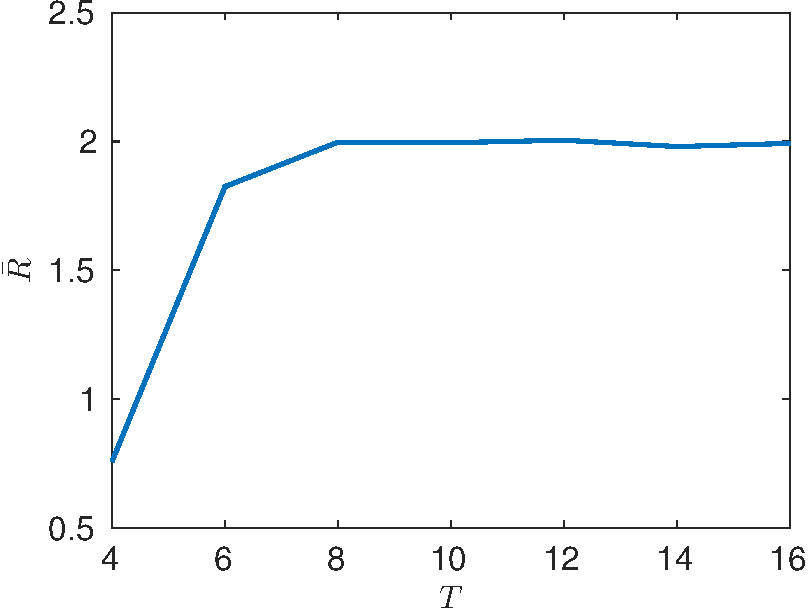
\includegraphics[width=.6\textwidth]{nonrealtime_throughput_T.pdf}
\caption{Network throughput versus interval length with non-real-time traffic.}
\label{nonrealtime_throughput_T}
\end{figure}

Figure \ref{realtime_throughput_T} shows the network throughput with different interval length with real-time traffic. Compared to the non-real-time case, the throughput with real-time traffic is even lower due to possible packet expiration. In other words, real-time traffic requires larger $T$ so that the effect of the expired packets can be mitigated. Besides, Figure \ref{realtime_throughput_T} serves as a useful reference for system design. For example, suppose both clients require a delivery ratio of 0.6. From Figure \ref{realtime_throughput_T}, we need to choose $T\geq 8$ to meet the requirement. 

\begin{figure}[htbp]
\centering
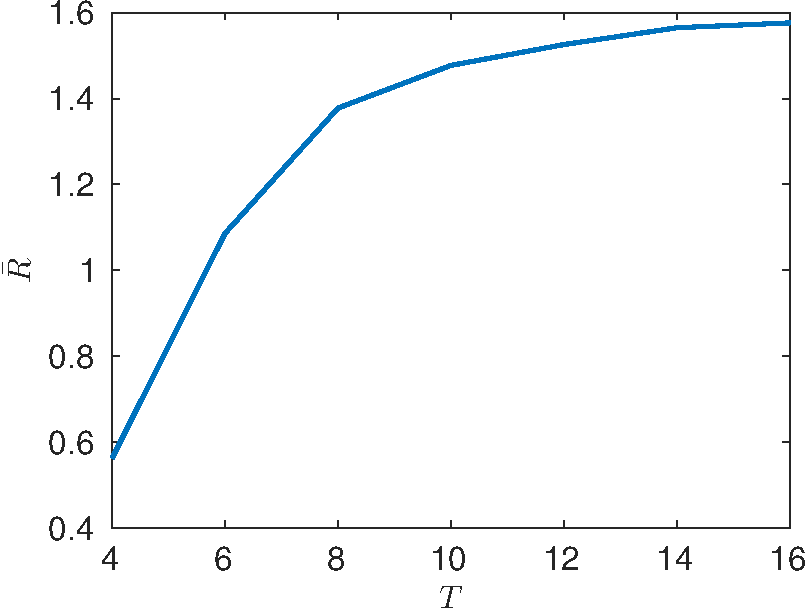
\includegraphics[width=.6\textwidth]{realtime_throughput_T.pdf}
\caption{Network throughput versus interval length with real-time traffic.}
\label{realtime_throughput_T}
\end{figure}

\subsection{Network Size and Polling Overhead}
\begin{figure}[htbp]
\centering
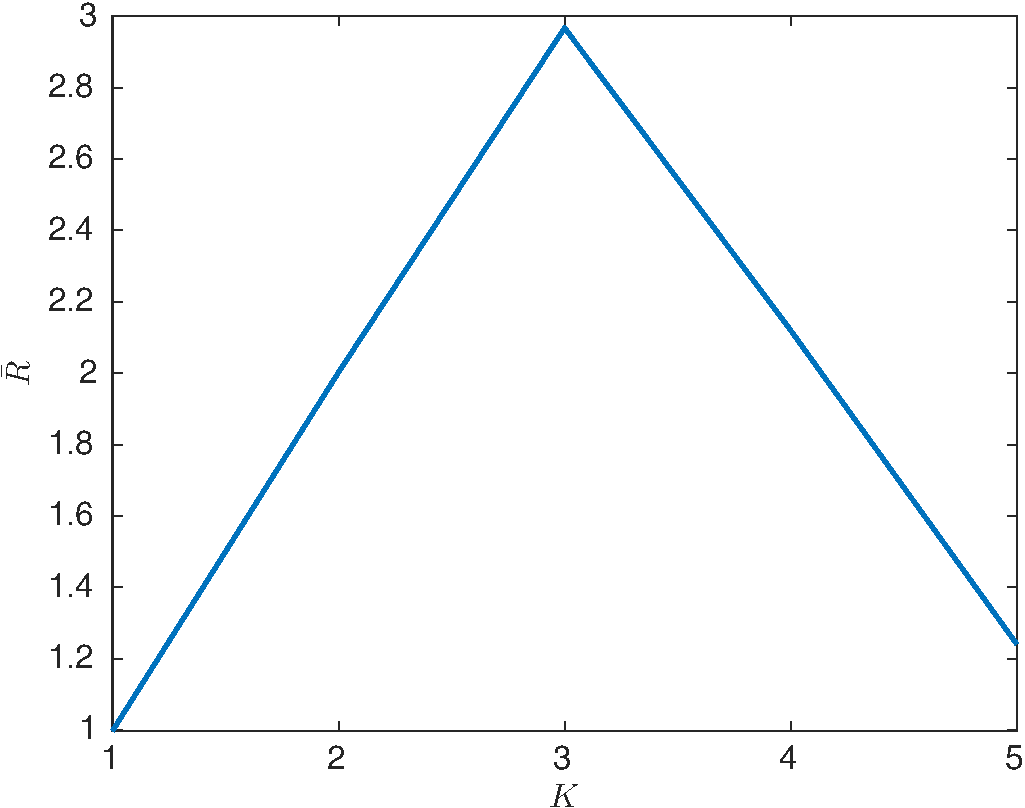
\includegraphics[width=.6\textwidth]{nonrealtime_throughput_K.pdf}
\caption{Network throughput versus network size with non-real-time traffic.}
\label{nonrealtime_throughput_K}
\end{figure}

\begin{figure}[htbp]
\centering
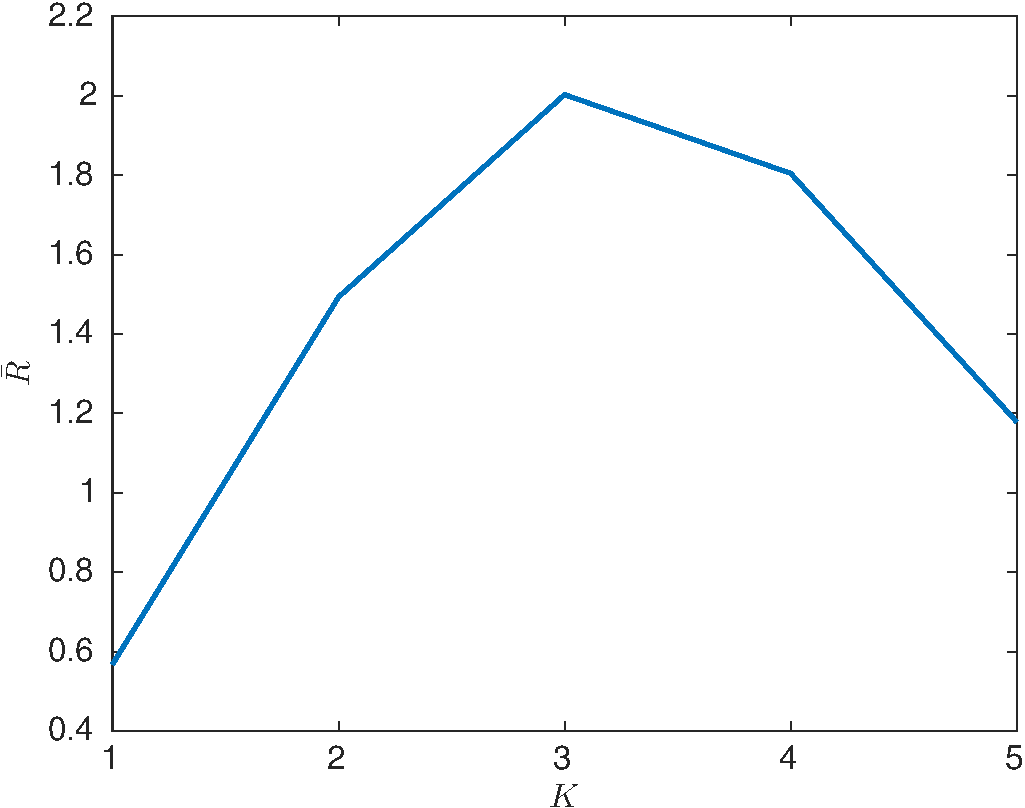
\includegraphics[width=.6\textwidth]{realtime_throughput_K.pdf}
\caption{Network throughput versus network size with real-time traffic.}
\label{realtime_throughput_K}
\end{figure}
We study the effect of network size on the polling overhead. Let $T = 10$, $N_{max}=2$, and channel reliability $p_1 = p_2 = 0.57$. Figure \ref{nonrealtime_throughput_K} shows the network throughput with non-real-traffic traffic for different network size. When $K$ grows from 1 to 3, the total throughput increases since the total traffic is not saturated yet. As $K$ exceeds 3, the network throughput drops significantly because the polling phase takes most of the time in an interval. Figure \ref{realtime_throughput_K} shows a similar pattern for the real-time case. 

In both scenarios, the network performance degrades severely with more clients. Hence, the baseline policy is not suitable for large networks due to the polling overhead. 

\section{Conclusion}
The baseline policy employs a simple polling scheme to collect queue information of the clients. Accordingly, the AP can be work-conserving in the scheduling phase. However, the channel utilization for data packets can be low due to the polling overhead. The overhead can degrade the network performance even more severely when the number of clients is large or the interval length is small. To mitigate this effect, we definitely need a smarter policy to accommodate uplink transmission with PCF.

\end{document}
